\section{System Architecture}\label{sec:sa}
Due to the fact that it is a web platform, the system is divided into two parts: the frontend and the backend. Frontend refers to the component of the system that will be visible to the user on the screen of a mobile device or computer. Whereas the back end refers to parts of the system or a program's code that allow it to operate and that cannot be accessed by a user. The back end is also called the data access layer of a system and includes any functionality that needs to be accessed and navigated to by digital means. The frontend is designed with more than 25 libraries including leading frontend library \textit{React.js}, \textit{MaterialUI}, \textit{Ant-Design}, \textbf{Bootstrap} and so on. These libraries are written on \textit{Javascript} programming language and is able to be integrated with any other programming language based backend libraries. We used more than 15 Javascript based frameworks such as \textit{Express Js}. For database management, we used \textit{MySQL}\footnotemark which is an open-source relational database management system. When a user tries to log in to the system with credentials, the the system catches the input data and send those to the backend first for certifying the authorized user. Backend functions then connect with the database server, and certifies the user.

All of the front-end information that a user sees is retrieved from the database and sent to the browser using backend functionalities. On the dashboard, different options are shown based on the roles of the users. CRUD (Creat, Read, Update, Delete) operations, that may be performed on the selections of the user from the dashboard. API\footnotemark (\textit{Application Programming Interface}) allows the backend to retrieve and alter data into the database through SQL queries. The following figure is a diagrammatic representation of the work-flow of the system.

Figure 13 illustrates the work flow of CU-OPAS(Chittagong University Online Payment and Attendance System). From the figure we can see that he system validates an user with his login credentials and shows different dashboard for students and teachers.


\footnotetext[5]{MySQL is the most popular Open Source Relational SQL database management system. MySQL is one of the best RDBMS being used for developing web-based software applications.}
\footnotetext[6]{An application programming interface is a connection between computers or between computer programs. It is a type of software interface, offering a service to other pieces of software. A document or standard that describes how to build or use such a connection or interface is called an API specification.}

\clearpage

\begin{figure}[H]
    \centering
    \label{fig:flowchart}
    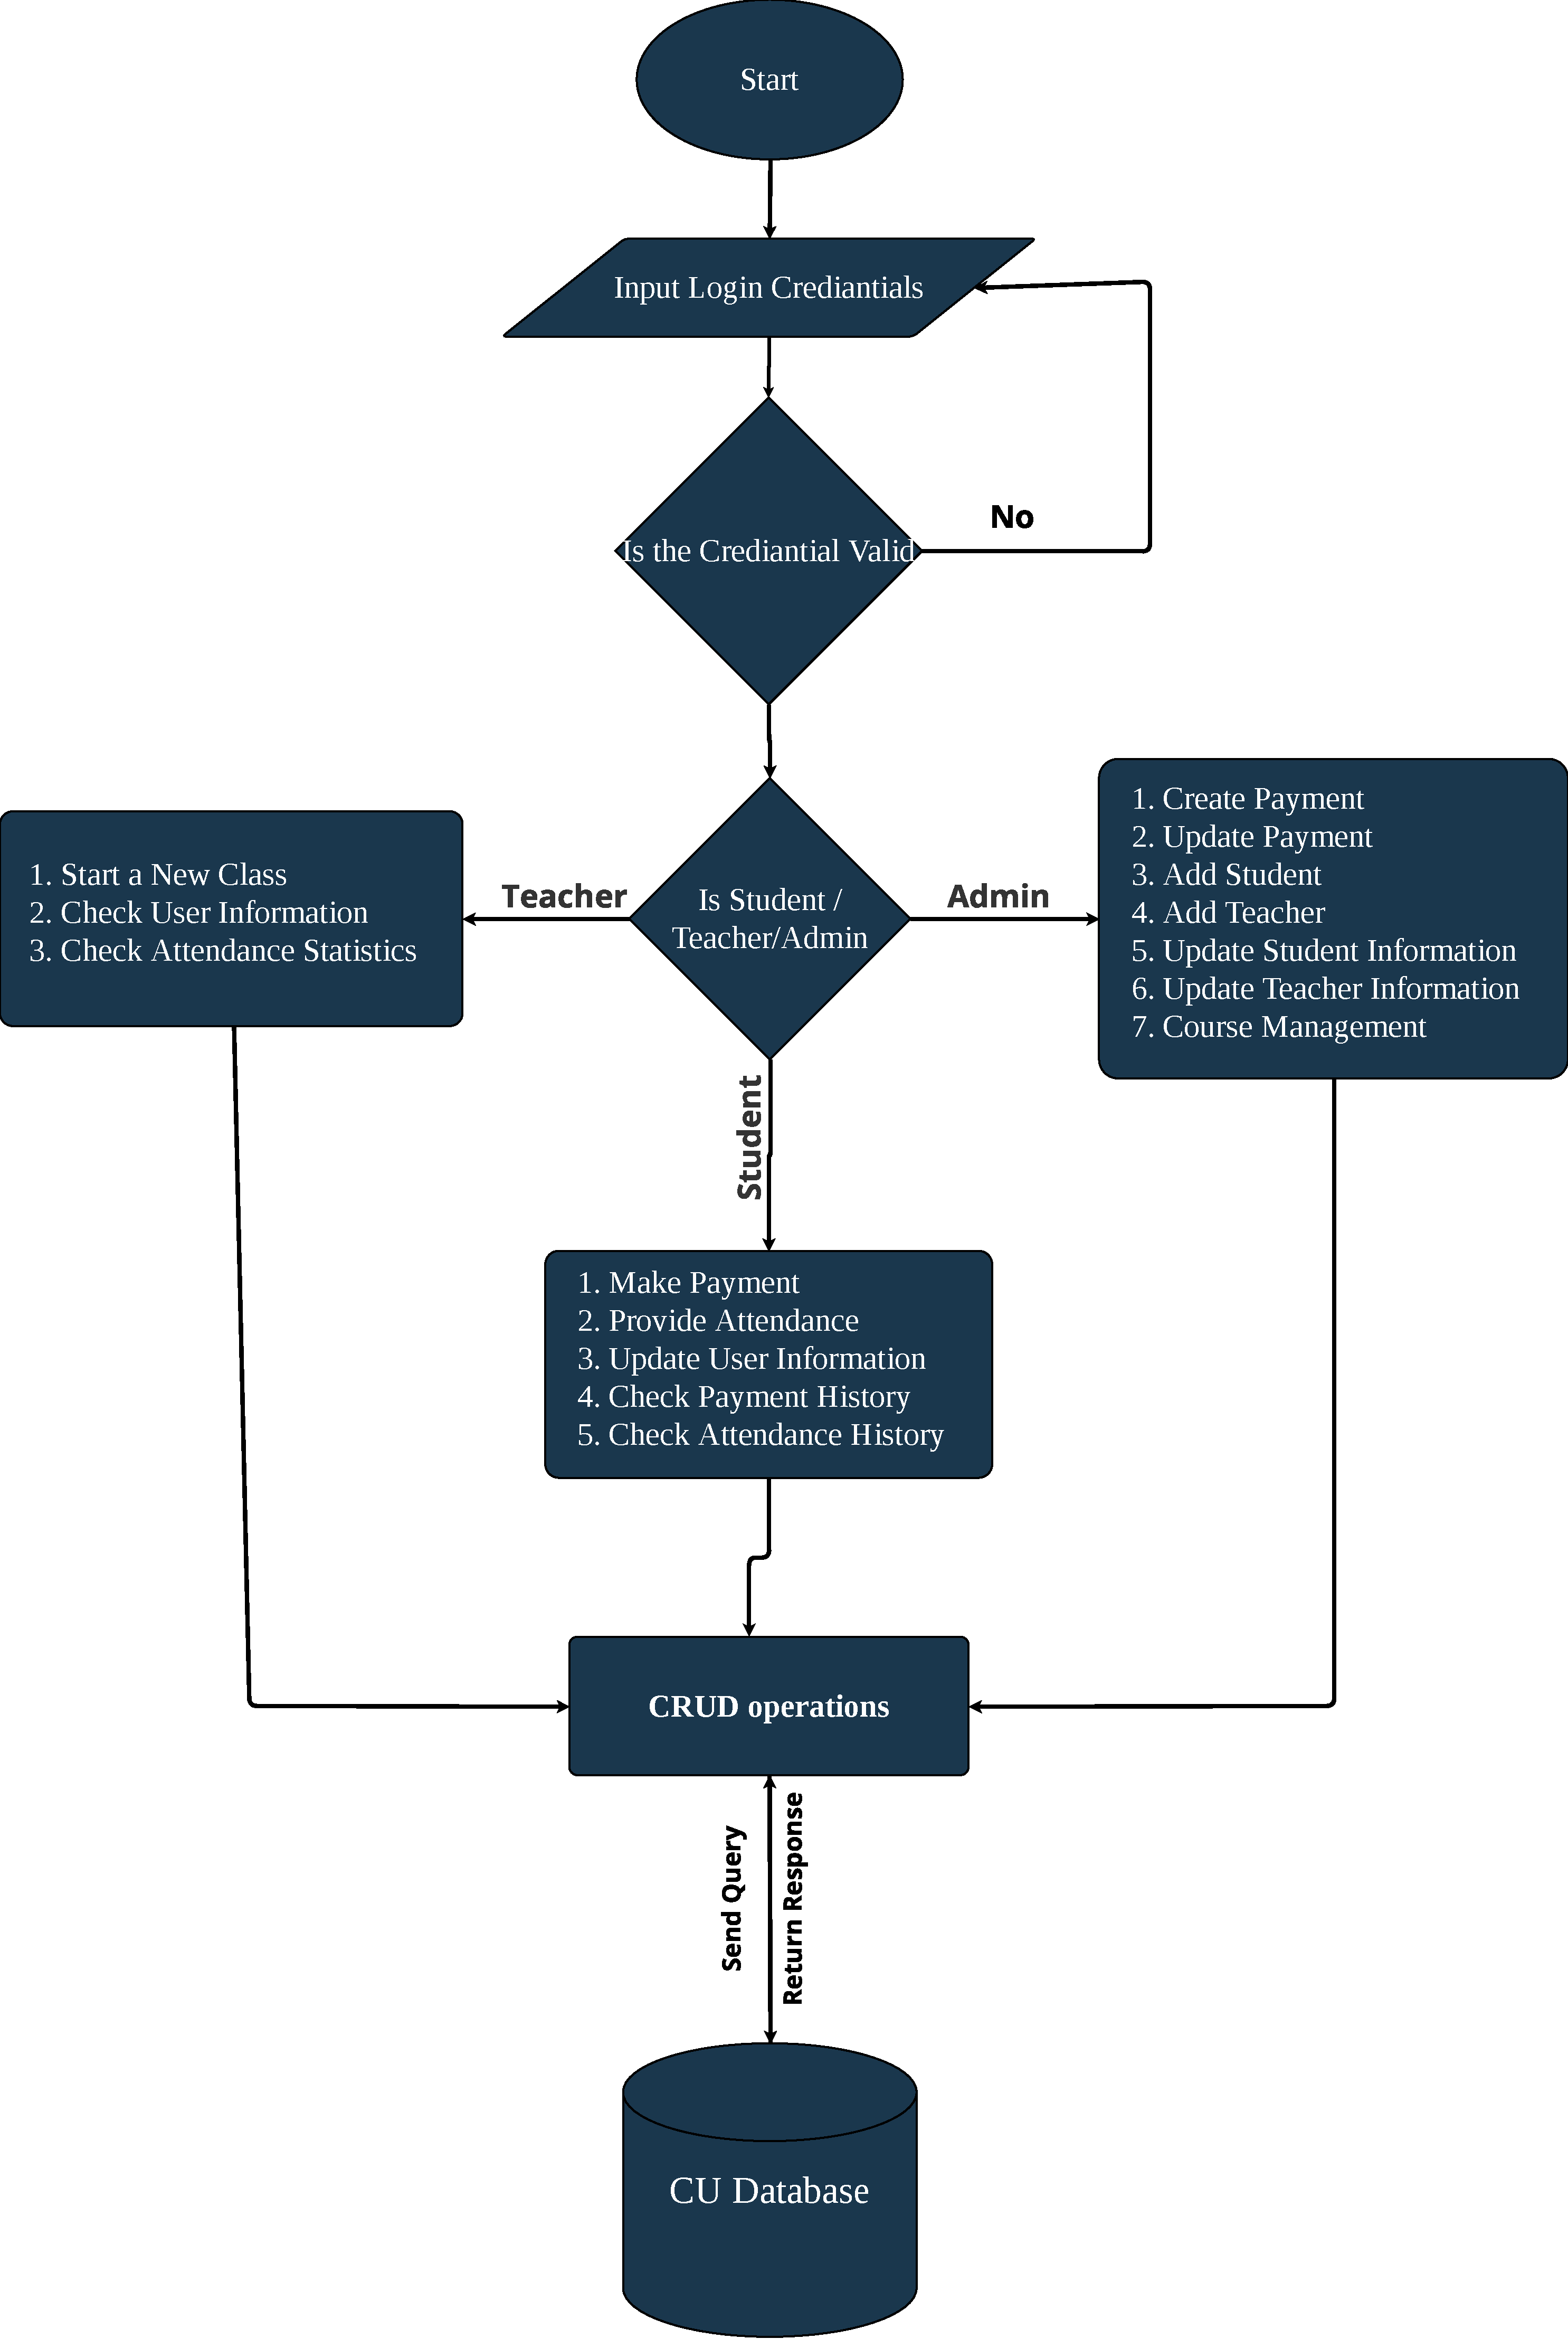
\includegraphics[height=15cm, width=1\textwidth]{images/flowchart}
    \caption{Work flow of the system}
\end{figure}

\clearpage